\documentclass[conference]{IEEEtran}
\IEEEoverridecommandlockouts

% Core math and fonts
\usepackage{amsmath,amssymb,amsfonts}
\usepackage{textcomp}
\usepackage{xcolor}

% Algorithms
\usepackage{algorithm}
\usepackage{algpseudocode}

% Graphics
\usepackage{graphicx}
\graphicspath{{Images/}}
\DeclareGraphicsExtensions{.eps,.jpeg,.png}

% Float and caption handling
\usepackage{float}
\usepackage{caption}
\usepackage{subfig}   % replaces subfigure

% References and URLs
\usepackage{cite}
\usepackage{url}

% Hyphenation
\hyphenation{op-tical net-works semi-conduc-tor IEEE-Xplore}

% Optional: highlights
\usepackage{soul}


% BEGIN PANAMA ADDITIONS: review markup and compilation support
\usepackage[T1]{fontenc}
\usepackage{etoolbox}
\definecolor{panamaaddition}{RGB}{0,135,45}
\newenvironment{panamaaddition}{\begingroup\color{panamaaddition}}{\endgroup}
% Preserve the supplied nonbreaking hyphen in both XeLaTeX and pdfLaTeX.
\ifdefined\XeTeXversion
  \catcode"2011=\active
  \protected\def‑{\mbox{-}}
  \catcode"2013=\active
  \protected\def–{\textendash}
  \catcode"2014=\active
  \protected\def—{\textemdash}
\else
  \DeclareUnicodeCharacter{2011}{\mbox{-}}
\fi
% Mark only the newly added PANAMA bibliography entry in green.
\makeatletter
\let\panama@originalbibitem\bibitem
\newcommand{\panama@bibcolor}[1]{%
  \ifstrequal{#1}{panama}{\color{panamaaddition}}{\color{black}}}
\renewcommand{\bibitem}{%
  \@ifnextchar[{\panama@optionalbibitem}{\panama@plainbibitem}}
\newcommand{\panama@plainbibitem}[1]{%
  \panama@bibcolor{#1}\panama@originalbibitem{#1}}
\newcommand{\panama@optionalbibitem}[2][]{%
  \panama@bibcolor{#2}\panama@originalbibitem[#1]{#2}}
\makeatother
% END PANAMA ADDITIONS: review markup and compilation support
\begin{document}

\title{Joint SAGIN Resource Allocation and MAPF for Digital Twin Supported Remote Robotic Applications}

\author{
    \IEEEauthorblockN{Irem~Bor-Yaliniz\IEEEauthorrefmark{1}, 
                      Arman~Dogru\IEEEauthorrefmark{2}, and 
                      Georges~Kaddoum\IEEEauthorrefmark{1}}
    \IEEEauthorblockA{\IEEEauthorrefmark{1}Department of Electrical Engineering, 
                      École de Technologie Supérieure (U. du Québec), Montréal, Canada\\
                      \{remziye-irem.bor-yaliniz, Georges.Kaddoum\}@etsmtl.ca}
    \IEEEauthorblockA{\IEEEauthorrefmark{2}Computer Science Department, 
                      University of Ottawa, Ottawa, Canada\\
                      adogr056@uottawa.ca}
}

\maketitle

\begin{abstract}
%%% BASIC
%Many automation scenarios, such as search \& rescue, defense and mining, operate in remote locations with unstable connectivity. In these scenarios, ubiquitous communications become a bottleneck for safe and efficient operations, where space-air-ground integrated networks (SAGIN) emerge as a critical enabler. However, the resulting system presents a complex resource allocation scenario involving SAGIN, optical inter-satellite links, and distributed computation to enable continuous digital twin (DT) verification. Specifically, this study investigates the co-design of DT resource distribution, optical backhaul and aerial RAN by proposing a semantic X-haul framework. We design a multi-agent path finding algorithm that is suitable for complex environments and utilize DTs to proactively control the operation. One aspect we test is emboided AI vs. cloud-based intelligence where the cost of unit robot and communications, as well as the reliability, latency and battery usage impacts are investigated. By investigating distributed vs. centralized DT and processing, we investigated delay, accuracy and energy cost. Finally, by feeding DT predictions into the trajectory planning for a low-altitude aerial access point, we demonstrate how the proposed intention sharing method can improve overall energy expenditure. 
%%% LONG
%In many automation scenarios, such as search and rescue, defense, and mining—operations are conducted in remote locations where network connectivity is often unstable. This lack of reliable communication becomes a bottleneck for safe and efficient operations. Space–air–ground integrated networks (SAGIN) have emerged as a key enabler in such environments. However, the resulting system introduces complex resource allocation challenges involving SAGIN, optical inter-satellite links, and distributed computation, particularly when continuous verification via digital twins (DTs) is required. This study investigates the co-design of DT resource distribution, optical backhaul, and aerial radio access networks (RAN) by proposing a semantic X-haul framework. We develop a multi-agent pathfinding algorithm suitable for complex environments and use DTs to proactively control system operation. A key comparison is drawn between embodied AI and cloud-based intelligence, evaluating trade-offs in unit robot and communication costs, reliability, latency, and battery usage. Furthermore, we analyze distributed versus centralized DT and processing architectures in terms of delay, accuracy, and energy cost. Finally, by feeding DT predictions into the trajectory planning of a low‑altitude aerial access point, we demonstrate that the proposed intention‑sharing method can significantly improve overall energy efficiency.
%%% 200 WORDS
Automation scenarios such as search and rescue, defense, and mining often operate in remote locations with unstable connectivity, making reliable communication a bottleneck for safe and efficient operations. Space–air–ground integrated networks (SAGIN) are a critical enabler, yet they introduce complex resource allocation challenges involving optical inter-satellite links and distributed computation for continuous digital twin (DT) verification. This study proposes a semantic X‑haul framework for the co‑design of DT resource distribution, optical backhaul, and aerial radio access networks. A multi‑agent pathfinding algorithm suitable for complex environments is developed, using DTs for proactive control. We compare embodied AI versus cloud‑based intelligence, evaluating trade‑offs in unit cost, reliability, latency, and battery usage. Additionally, distributed and centralized DT architectures are analyzed in terms of delay, accuracy, and energy cost. Finally, by feeding DT predictions into the trajectory planning of a low‑altitude aerial access point, we demonstrate that an intention‑sharing method can improve overall energy expenditure. The results highlight the benefits of jointly designing computation and communications from algorithm design to resource allocation and exemplifies the unavoidable convergence between them.


\end{abstract}

\begin{IEEEkeywords}
Satellite communications, robotics, cyber-physical systems, space-air-ground integrated networks, multi-agent path finding, 6G.
\end{IEEEkeywords}
\begin{figure}[h!]
    \centering
    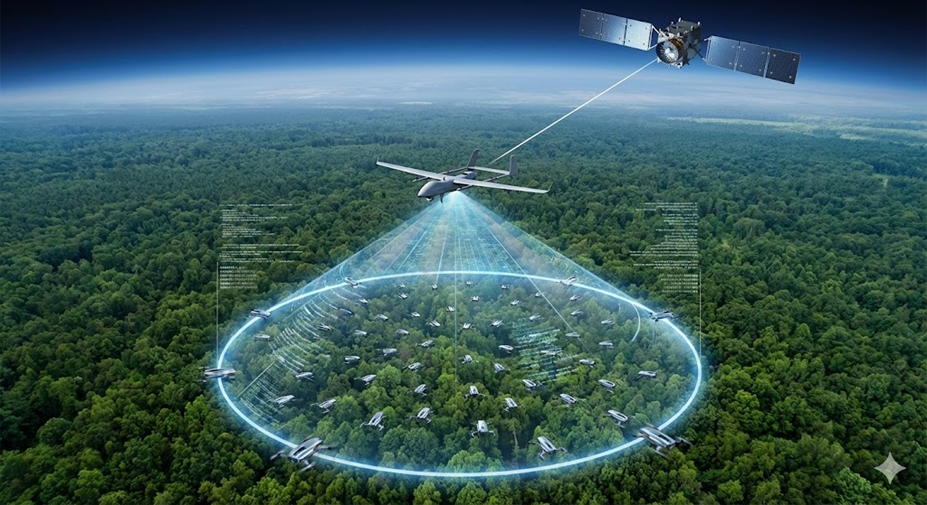
\includegraphics[width=\linewidth]{image.png}
    \caption{System model including SAGIN elements and cyber-physical systems operation in a remote location}
    \label{fig:placeholder}
\end{figure}

\section{Introduction}
\begin{itemize}
    \item Digital Twins: The study in~\cite{dt_resource} proposes a method to utilize digital twins (DTs) for multi-domain resource management of SAGIN networks for ISAC purposes. This study also considers mapping errors of DTs due to imperfect sensing.   
    \item SAGIN 
    \item Ray-tracing
    \item Outage analysis: The studies in~\cite{o_altitude,o_cfmimo,o_fso} provide outage analysis under a variety of system settings from CF-MIMO to FSO connectivity for SAGIN, where UAV is used either as a relay or access point. However, none of these articles take advantage of DTs.
    The study in \cite{o_fso} models satellite-UAV links as FSO and UAV-UE as RF links with MISO and Nakagami-m fading. This article provides analytical outage analysis under several practical constraints, such as outdated CSI and misalignment of FSO transcievers. The study in~\cite{o_altitude} investigates the affects of UAV position in the outage probability, which could be useful to analyze the affect of incorrect position estimation. The study in~\cite{o_cfmimo} provides uplink analysis and provides a method to optimize ground users' power transmit levels, which can be useful.
\end{itemize}



% BEGIN PANAMA ADDITIONS: algorithmic scope
\begin{panamaaddition}
This work extends PANAMA's centralized training with decentralized execution
framework~\cite{panama} to distinguish communication delay from physical robot
motion. During mission execution, delayed guidance and peer reports change the
information available to a robot, while its local sensing and previously
deployed policy remain available. During learning, delayed experience uploads
restrict the learner's received data, and delayed model deployments cause
robots to act with different versions of the shared policy. We formulate these
effects through message timestamps, receiver caches, and model versions. The
transport supplies the corresponding delays; their LEO-specific derivation is
separate from the algorithm developed here.
\end{panamaaddition}
% END PANAMA ADDITIONS: algorithmic scope

\section{System Model}
The system is as follows.

Let $\mathcal{N} = \{1, 2, \dots, N\}$ denote the set of ground robots. Each robot $i \in \mathcal{N}$ generates a computationally intensive task modeled as a tuple $D_i = \{s_i, c_i, \tau_i\}$, where $s_i$ is the input data size in bits, $c_i$ is the required CPU cycles per bit, and $\tau_i$ is the maximum tolerable latency in seconds.

The system relies on the following decision variables:
\begin{itemize}
    \item $x_i \in \{0, 1\}$: The offloading decision indicator. $x_i = 1$ if task $i$ is processed locally at the Drone-AP; $x_i = 0$ if the task is relayed to the Cloud.
    \item $P_i \ge 0$: The transmit power of robot $i$ on the Ground-to-Air (G2A) link.
    \item $f_{D,i} \ge 0$: The Drone CPU frequency allocated to task $i$.
    \item $f_{C,i} \ge 0$: The Cloud CPU frequency allocated to task $i$.
\end{itemize}
\subsection{Ground-to-Air (G2A) Channel}
The G2A channel between the ground robots and the Drone-AP is modeled using a probabilistic Line-of-Sight (LoS) and Non-Line-of-Sight (NLoS) framework. The path loss for robot $i$, denoted $L^{\text{G2A}}_i$ in dB, is expressed as:
\begin{equation}
L^{\text{G2A}}_i = 20 \log_{10}\left(\frac{4\pi f_c d_i}{c}\right) + \eta
\end{equation}
where $d_i$ is the 3D distance between robot $i$ and the drone, $f_c$ is the carrier frequency, $c$ is the speed of light, and $\eta$ is the additional attenuation factor depending on whether the link is LoS ($\eta_{\text{LoS}}$) or NLoS ($\eta_{\text{NLoS}}$).\hl{Add Al-Hourani's channel model here!!}

The achievable uplink data rate is given by:
\begin{equation}
R^{\text{G2A}}_i = B_{\text{G2A}} \log_2 \left( 1 + \frac{P_i 10^{-L^{\text{G2A}}_i/10}}{N_0 B_{\text{G2A}}} \right)
\end{equation}
where $B_{\text{G2A}}$ is the channel bandwidth and $N_0$ is the noise power spectral density.\hl{take the channel bw value from simulator!}

\subsection{Air-to-Space (A2S) Channel}
The backhaul link from the Drone-AP to the LEO satellite relies on a strong LoS channel. The path loss $L^{\text{A2S}}$ incorporates Free Space Path Loss and atmospheric attenuation $\xi_{\text{atm}}$:
\begin{equation}
L^{\text{A2S}} = 20 \log_{10}\left(\frac{4\pi f_{\text{sat}} d^{t}_{\text{sat}}}{c}\right) + \xi_{\text{atm}},
\end{equation}
where $d^{t}_{\text{sat}}$ indicates the distance between the satellite and the UAV-BS at time $t$.\hl{consider using $\bar{d}$ to indicate average d while uav and sat are associated!}

The achievable A2S data rate for relayed tasks is:
\begin{equation}
R^{\text{A2S}}_i = B_{\text{A2S}} \log_2 \left( 1 + \frac{P_D |g|^2 10^{-L^{\text{A2S}}/10}}{N_0 B_{\text{A2S}}} \right)
\end{equation}
where $P_D$ is the transmission power of the Drone-AP and $g$ models the Rician fading component.\hl{find the bw value and exact channel parameters!}

\hl{We need to add space-air and air-to-ground downlink parameters. Only changing the tx power may be sufficient!}

\subsection{Latency Model}
The latency experienced by task $i$ depends on the offloading decision. If computed at the Drone-AP ($x_i = 1$):
\begin{equation}
T_{i, \text{Drone}} = \frac{s_i}{R^{\text{G2A}}_i} + \frac{s_i c_i}{f_{D,i}}
\end{equation}

If the task is relayed to the Cloud ($x_i = 0$):
\begin{equation}
T_{i, \text{Cloud}} = \frac{s_i}{R^{\text{G2A}}_i} + \frac{s_i}{R^{\text{A2S}}_i} + T_{\text{prop}} + \frac{s_i c_i}{f_{C,i}}
\end{equation}
where $T_{\text{prop}} \approx 2 \bar{d}_{\text{sat}} / c$ represents the satellite round-trip propagation delay by using the average of the distance between the UAV and the satellite while associated. The total latency for task $i$ is thus:
\begin{equation}
T_i = x_i T_{i, \text{Drone}} + (1 - x_i) T_{i, \text{Cloud}}
\end{equation}

\subsection{Energy Consumption Model}
The transmission energy consumed by robot $i$ is:
\begin{equation}
E^{\text{tx}}_i = P_i \frac{s_i}{R^{\text{G2A}}_i}
\end{equation}\hl{confirm that this needs to be fixed for 3D placement}
The energy expended by the Drone-AP encompasses local computation and relaying transmissions. Let $\kappa_D$ denote the \hl{effective switched capacitance} of the drone's computing architecture\hl{is this well known and widely used? how about GOP?}. The drone energy cost for task $i$ is:
\begin{equation}
E_{\text{Drone}, i} = x_i \kappa_D (f_{D,i})^2 s_i c_i + (1 - x_i) P_D \frac{s_i}{R^{\text{A2S}}_i}
\end{equation}
% BEGIN PANAMA ADDITIONS: communication and information state
\begin{panamaaddition}
\subsection{Timestamped Communication and Information Age}
Let $n\in\mathbb{N}_0$ index joint robot actions, with decision time
$t_n=n\Delta$ and step duration $\Delta>0$. Robot $i$ occupies grid position
$\mathbf{q}_i(n)$ and has a known goal $\mathbf{g}_i$. Its physical state is
distinct from the information stored at a remote processor or another robot.
Each message $m$ carries its source timestamp $g_m$, sequence or model version
$\nu_m$, and complete payload. Its receiver obtains that payload at
\begin{equation}
 b_m=g_m+\delta_m,\qquad \delta_m\geq0,
 \label{eq:panama-arrival}
\end{equation}
where $\delta_m$ is the end-to-end delay supplied by the communication
transport. A message with no completed delivery has $b_m=+\infty$. The
algorithm does not prescribe a distribution for $\delta_m$ or a handover
schedule. A subsequent LEO model determines these arrival times.

For a receiver stream $f$, let $\mathcal{M}_i^f(t_n)$ contain its messages
fully received by $t_n$. We consider task guidance $f=G$, peer intentions
$f=I_j$, and peer priorities $f=P_j$, for $j\in\mathcal{N}$. The accepted
message and corresponding cache are
\begin{align}
 m_i^{f,*}(n)&=\operatorname*{arg\,max}_{m\in\mathcal{M}_i^f(t_n)}
                         (g_m,\nu_m),\label{eq:panama-cache}\\
 \widehat{z}_i^f(n)&=z_{m_i^{f,*}(n)},
\end{align}
where the maximum uses lexicographic timestamp--version order. An initial
mission briefing initializes every cache at $t_0$. If no newer message
arrives, the stored value persists. An out-of-order older message cannot
overwrite a newer accepted cache.

A relayed or aggregated payload also retains the timestamp of each source
report, denoted $s_m^f$. Its information age is
\begin{equation}
 A_i^f(n)=t_n-s_{m_i^{f,*}(n)}^f.
 \label{eq:panama-age}
\end{equation}
For guidance, this is the timestamp of the robot state used to compute the
route. For intentions and priorities, it is the timestamp of the relevant
peer report. A newly received message can therefore contain old source
information. Aggregated peer age is the maximum of the included source ages.

Robots communicate through the UAV. For peer $j$ and receiver $i$, the
transport delay $\delta_{j\rightarrow i}^{f}$ covers the report and returned
update along the selected processing route. UAV processing permits local
exchange without the satellite backhaul, whereas cloud processing requires
backhaul forwarding. A cutoff prevents new deliveries on the affected route
and increases cache age. It does not remove the last received peer intention
or replace the robot's known goal. UAV positioning uses its own latest
received robot-position reports, $\widehat{\mathbf{q}}_i^U(t)$, rather than
instantaneous global positions unavailable to that receiver.

\subsection{Physical State and Available Decision Information}
Self-position, locally sensed obstacles, and visible robot positions remain
current at each action. Communication affects only the designated cached
guidance, intentions, or priorities. The simulator resolves physical
collisions, calculates task rewards, and checks mission completion using the
true state. Cached priorities modify observation construction, not the
physical transition rule. An age value is recorded for analysis; it is not
an additional input to the retained policy. Thus the delay extension preserves
the policy input dimensions while changing the timestamps of selected inputs.
\end{panamaaddition}
% END PANAMA ADDITIONS: communication and information state

\section{Optimization Problem Formulation}

We formulate a Mixed-Integer Non-Linear Programming (MINLP) problem to jointly optimize the routing decisions, transmit powers, and computational resource allocations. The objective is to minimize a weighted sum of the robots' transmission energy, the system latency, and the drone's energy load. Let $\omega_1, \omega_2, \omega_3$ be user-defined weighting coefficients such that $\omega_1 + \omega_2 + \omega_3 = 1$.


The problem is mathematically formulated as:
\begin{equation}
\min_{\mathbf{x}, \mathbf{P}, \mathbf{f}_D, \mathbf{f}_C} \sum_{i=1}^N \left[ \omega_1 E^{\text{tx}}_i + \omega_2 T_i + \omega_3 E_{\text{Drone}, i} \right]
\end{equation}

\textbf{Subject to:}
\begin{align}
& T_i \le \tau_i, \quad \forall i \in \mathcal{N} \label{eq:c1} \\
& 0 \le P_i \le P^{\text{max}}_{\text{robot}}, \quad \forall i \in \mathcal{N} \label{eq:c2} \\
& \sum_{i=1}^N x_i f_{D,i} \le F^{\text{max}}_{\text{Drone}} \label{eq:c3} \\
& \sum_{i=1}^N (1 - x_i) f_{C,i} \le F^{\text{max}}_{\text{Cloud}} \label{eq:c4} \\
& f_{D,i} \ge 0, \quad f_{C,i} \ge 0, \quad \forall i \in \mathcal{N} \label{eq:c5} \\
& x_i \in \{0, 1\}, \quad \forall i \in \mathcal{N} \label{eq:c6}
\end{align}

Constraint \eqref{eq:c1} ensures that tasks are processed within their maximum tolerable latency limit. Constraint \eqref{eq:c2} bounds the ground robots' transmit power. Constraints \eqref{eq:c3} and \eqref{eq:c4} ensure that the total allocated CPU frequencies do not exceed the respective maximum capacities of the Drone-AP and the Cloud server. Finally, constraints \eqref{eq:c5} and \eqref{eq:c6} define the bounds and domains of the continuous and binary variables, respectively.


% BEGIN PANAMA ADDITIONS: PANAMA under communication delay
\begin{panamaaddition}
\subsection{PANAMA Policy with Cached Mission Information}
We use PANAMA's shared dual-stream action-value network, Double DQN learner,
prioritized experience replay (PER), task reward, and exploration mechanism~\cite{panama}.
Nominal learning parameters follow Table~III of PANAMA, including discount
$\gamma=0.99$, AdamW learning rate $10^{-4}$, minibatch size $M=64$, replay
capacity $2\times10^6$, and target mixing coefficient $\eta_{\rm tar}=0.005$.
The communication mechanism introduces no additional reward, imitation policy,
or recovery action. We consider the task-policy channels for obstacles,
visible robots, and communicated intentions, with UAV-mediated transport.
Terrestrial radio maps and additional SNR-based shaping are outside this
algorithmic extension.

An accepted guidance payload contains an absolute A* route
$\mathcal{P}_i=(\mathbf{w}_{i,0},\ldots,\mathbf{w}_{i,L})$ and reported
distance $\widehat{d}_i$. The processor computes the route from the position
in the generating report to $\mathbf{g}_i$, using the static obstacle map.
While awaiting another guidance message, robot $i$ consumes waypoints it has
already reached and retains the remaining absolute route. On late delivery,
it also removes waypoints reached since that route's source timestamp.
It neither recomputes A* locally nor translates old relative offsets as if
they referred to its current position. The reported distance remains the
received value until another guidance update arrives.

Let $\widehat{\mathbf{w}}_{i,k}(n)$ denote the $k$th remaining waypoint.
The waypoint features use current self-position,
\begin{equation}
 \widehat{\mathbf{u}}_{i,k}(n)=
 \operatorname{clip}_{[-1,1]}
 \!\left(\frac{\widehat{\mathbf{w}}_{i,k}(n)-\mathbf{q}_i(n)}{h}\right),
 \label{eq:panama-waypoint}
\end{equation}
where clipping is componentwise, $h=7$ is the PANAMA field-of-view radius,
and $k\in\{1,\ldots,K\}$ with $K=5$. Unavailable waypoints contribute zero
features. The retained task vector concatenates normalized reported distance,
the local ever-reached-goal flag $f_i^g(n)$, and these waypoint pairs:
\begin{equation}
 \widehat{\mathbf{v}}_i(n)=
 (\widehat{d}_i/d_i^0,\ f_i^g(n),\
  \widehat{\mathbf{u}}_{i,1},\ldots,\widehat{\mathbf{u}}_{i,K}),
 \label{eq:panama-vector}
\end{equation}
with distance clipped to $[0,1]$ and the initial briefing distance $d_i^0$
as normalizer. A nonpositive or nonfinite normalizer uses the map's larger
dimension, as in the retained task implementation. The goal remains known
even when the route or its reported distance is stale.

Let $\widehat{\mathcal{I}}_{j\rightarrow i}(n)$ be the last received absolute
path segment of peer $j$, and let $\widehat{\rho}_{j\rightarrow i}(n)$ be its
received priority, with smaller values indicating higher priority. Robot $i$
forms the intention channel from peers whose received priority precedes its
own received priority, subject to PANAMA's communication range, local
field of view, and received completion flag. A cached path cell
$\mathbf{w}$ is placed relative to the current $\mathbf{q}_i(n)$.
Writing $\mathcal{R}_i(n)$ for the eligible peers within PANAMA's communication
range and $\widehat{f}_{j\rightarrow i}^{g}$ for their received completion
flags, the contributing set is
\begin{equation}
 \mathcal{H}_i(n)=\left\{j\in\mathcal{R}_i(n)\setminus\{i\}:
 \begin{array}{l}
  \widehat{\rho}_{j\rightarrow i}<\widehat{\rho}_{i\rightarrow i},\\
  \widehat{f}_{j\rightarrow i}^{g}=0
 \end{array}\right\}.
 \label{eq:panama-peer-set}
\end{equation}
For a relative field-of-view cell $\mathbf{z}$, the intention-channel value is
\begin{equation}
 \widehat{O}_i^I(\mathbf{z},n)=\mathbf{1}\!\left\{
 \mathbf{q}_i(n)+\mathbf{z}\in
 \bigcup_{j\in\mathcal{H}_i(n)}\widehat{\mathcal{I}}_{j\rightarrow i}(n)
 \right\}.
 \label{eq:panama-intention-mask}
\end{equation}
Communication loss therefore leaves the peer's old segment in the observation,
while local sensing can still reveal its actual nearby position. Denoting
fresh obstacle and robot channels by $O_i^{\rm obs}(n)$ and
$O_i^{\rm rob}(n)$, the policy input is
\begin{equation}
 \widehat{o}_i(n)=
 \big([O_i^{\rm obs},O_i^{\rm rob},\widehat{O}_i^I],
       \widehat{\mathbf{v}}_i\big).
 \label{eq:panama-observation}
\end{equation}
Each robot continues choosing among north, south, east, west, and wait using
this available input. Communication unavailability does not itself mandate
waiting or insert an external collision-recovery controller.

\subsection{Received Experiences and Continued Learner Operation}
After joint action $n$, robot $i$ produces the complete transition
\begin{equation}
 \zeta_i(n)=
 (\widehat{o}_i(n),a_i(n),r_i(n+1),
  \widehat{o}_i(n+1),z(n+1)),
 \label{eq:panama-transition}
\end{equation}
where $z$ is the task simulator's terminal flag. The tuple is captured at
$t_{n+1}$ together with robot, episode, joint-step, and deployed-version
identifiers. Upload delay changes only its arrival time,
\begin{equation}
 b_i^E(n)=t_{n+1}+\delta_i^E(n).
 \label{eq:panama-upload}
\end{equation}
The transition's observations, action, reward, and terminal flag remain tied
to their generating step, regardless of later robot motion or weight updates.

At learner time $t$, the received subset of the $N$ expected transitions
from joint action $n$ is
\begin{equation}
 \mathcal{U}_n(t)=\{i\in\mathcal{N}:b_i^E(n)\leq t\}.
 \label{eq:panama-subset}
\end{equation}
The replay buffer contains only fully received transitions, subject to its
capacity and curriculum-phase retention rule. In particular,
\begin{equation}
 \mathcal{B}(t)\subseteq
 \bigcup_{n:\,t_{n+1}\leq t}
 \{\zeta_i(n):i\in\mathcal{U}_n(t)\}.
 \label{eq:panama-replay}
\end{equation}
The set on the right ranges over all generated joint actions. The learner
does not require $\mathcal{U}_n(t)=\mathcal{N}$ before learning. It can use
received experiences from unaffected robots and previously delivered replay
samples while other uploads remain pending. If all current uploads are
delayed, existing replay still supports updates. A learning opportunity is
skipped only when insufficient replay data are available. Late experiences
from a completed curriculum phase are excluded from the new phase's replay.

For each sampled transition $\zeta=(o,a,r,o',z)$, the retained Double DQN
target and weighted Huber loss are
\begin{align}
 a_\zeta^*&=\operatorname*{arg\,max}_{a'}Q_\theta(o',a'),\\
 y_\zeta&=r+\gamma(1-z)Q_{\theta^-}(o',a_\zeta^*),\\
 \mathcal{L}(\theta)&=\frac{1}{M}
       \sum_{\zeta\in\mathcal{J}(t)}
       w_\zeta\,\ell_{\rm H}\big(Q_\theta(o,a)-y_\zeta\big),
 \label{eq:panama-loss}
\end{align}
where $\mathcal{J}(t)$ is a PER minibatch from $\mathcal{B}(t)$ and
$w_\zeta$ is its importance-sampling weight. AdamW updates $\theta$ and the
target follows
$\theta^-\leftarrow(1-\eta_{\rm tar})\theta^-+\eta_{\rm tar}\theta$.
The delayed upload can change data availability and replay age, but does not
replace the learning rule with an update based on incomplete tuples.
The learner is off-policy: an experience collected with an older deployed
version remains a complete training sample, and the learner evaluates its
target with the current policy and target networks. Recording the generating
version permits analysis of this mismatch without requiring every robot to
hold the latest model before a learner update.

\subsection{Complete Model Deployment and Per-Robot Staleness}
Let $\Theta^\ell$ be the immutable complete model snapshot published at time
$u_\ell$, with increasing publication version $\ell$. For robot $i$, its
completed downlink arrival is
\begin{equation}
 b_i^W(\ell)=u_\ell+\delta_i^W(\ell).
 \label{eq:panama-download}
\end{equation}
Immediately before action $n$, robot $i$ uses
\begin{align}
 v_i(n)&=\max\{\ell:b_i^W(\ell)\leq t_n\},\\
 \widetilde{\theta}_i(n)&=\Theta^{v_i(n)},
 \label{eq:panama-deployed}
\end{align}
with a complete initial model available at $t_0$. A receiver installs a newer
snapshot atomically after full reception, before its next action. It never
mixes layers, partially received parameters, or components of two versions.
A late snapshot with $\ell\leq v_i(n)$ cannot roll the deployed model back.

The action is selected by the standard epsilon-greedy rule,
\begin{align}
 a_i^*(n)&=\operatorname*{arg\,max}_{a\in\mathcal{A}}
     Q_{\widetilde{\theta}_i(n)}(\widehat{o}_i(n),a),\\
 \pi_i(a\mid\widehat{o}_i;n)&=\frac{\epsilon_n}{|\mathcal{A}|}
       +(1-\epsilon_n)\mathbf{1}\{a=a_i^*(n)\}.
 \label{eq:panama-action}
\end{align}
Exploration retains PANAMA's schedule and depends on generated environment
steps, not on delivered experience counts. A missing downlink update leaves
$\widetilde{\theta}_i(n)$ unchanged while the robot continues acting.
Other robots can install newer snapshots independently, and the centralized
learner can continue optimizing its current model. Publications occur every
$H$ generated joint actions, with the same $H$ in all learning conditions.

Let $\ell_{\rm pub}(t_n)$ be the latest published version. We separately
measure model-version lag and model age,
\begin{align}
 L_i^W(n)&=\ell_{\rm pub}(t_n)-v_i(n),\\
 A_i^W(n)&=t_n-u_{v_i(n)}.
 \label{eq:panama-model-age}
\end{align}
Experience delivery age is $b_i^E(n)-t_{n+1}$; replay age at sampling time
$t$ is $t-t_{n+1}$. These quantities distinguish old policy execution from
old learning data without treating either as a halted mission.

\subsection{Operation and Separation of Communication Effects}
Algorithm~\ref{alg:panama-delay} summarizes the event-driven execution.
The flag $\chi_L$ equals one when learning is enabled and zero during
frozen-policy inference.
One learning opportunity follows each generated joint action. Generated
steps, delivered experiences, completed learner updates, and published models
are counted independently. Delayed uploads cannot redefine the step counter
or prevent other robots from contributing experiences. The simulator advances
its communication clock with robot actions and processes arrivals at their
timestamps, without a wall-clock sleep representing communication delay.

\begin{algorithm}[t]
\color{panamaaddition}
\captionsetup{font={color=panamaaddition},labelfont={color=panamaaddition}}
\caption{PANAMA with timestamped information and learning transport}
\label{alg:panama-delay}
\begin{algorithmic}[1]
\Require Initial caches, model $\Theta^0$, replay $\mathcal{B}$, $\chi_L$
\For{each generated joint action $n$}
  \State Process completed arrivals up to decision time $t_n$
  \State Accept newer information and complete model versions
  \For{each robot $i\in\mathcal{N}$}
    \State Sense locally and consume reached cached waypoints
    \State Construct $\widehat{o}_i(n)$ and act with $\Theta^{v_i(n)}$
  \EndFor
  \State Apply joint action using the true physical transition
  \State Advance event time and process completed arrivals
  \For{each robot $i\in\mathcal{N}$}
    \State Submit timestamped mission reports to the transport
    \State Capture and queue the complete $\zeta_i(n)$
  \EndFor
  \State Insert newly received eligible experiences into $\mathcal{B}$
  \If{$\chi_L=1$ and $|\mathcal{B}|\geq M$}
    \State Perform one standard PER/Double DQN update
  \EndIf
  \If{$\chi_L=1$ and $n+1$ is a multiple of $H$}
    \State Publish and queue complete snapshot $\Theta^{\ell+1}$
  \EndIf
\EndFor
\end{algorithmic}
\end{algorithm}

For frozen-policy mission analysis, all robots use one fixed snapshot and
learning is disabled. The transport changes only the selected guidance,
intention, or priority streams; unselected inputs remain current. For
learning-transport analysis, mission information remains current and we
compare immediate upload and deployment with delayed upload, delayed
deployment, and their combination. The same initialization and nominal PANAMA
parameters apply to those learning conditions. This separation attributes
mission effects to stale communicated information and learning effects to
received-data or deployed-model staleness. It makes no assumption that a
communication delay necessarily reduces success.
\end{panamaaddition}
% END PANAMA ADDITIONS: PANAMA under communication delay

% This include was referenced by the supplied main file but was not attached.
% Deliberately empty: no simulation section or results have been invented.

\bibliography{library.bib}
\bibliographystyle{IEEEtran}
\end{document}
